% Quelques mots sur le m�tier:
% + rappel sur les fonctions
% + rappel sur les distributions
% + rappel sur les convergences
% + rappel sur les stats
\documentclass[8pt]{beamer}

\setbeamertemplate{background canvas}[vertical shading][bottom=cyan!10,top=blue!10]

\usetheme{Warsaw}
\usefonttheme[onlysmall]{structurebold}

% pour le fichiers .pdf
\usepackage{graphicx}
\usepackage{color}
% pour les fichiers .png
% \usepackage{pgf,pgfarrows}
% \usepackage{pgf,pgfarrows}
\usepackage{amsmath,amssymb}
\usepackage[latin1]{inputenc}
\usepackage[T1]{fontenc}
%\usepackage[french]{babel}
\usepackage{textcomp}
\usepackage{Math_Notations}
\usepackage{multitoc}
\usepackage{mdwtab}
\setbeamercovered{dynamic}
\DeclareMathOperator*{\argmin}{argmin}

\title[OpenTURNS Developer Training]{OpenTURNS Developer Training\\Probabilistic uncertainty propagation}
\author[OpenTURNS Consortium, 2019]{
  Trainer : R�gis LEBRUN\\
  EADS/IW/SE/AM \\
  regis.lebrun@eads.net
}

\date[March 22-25th 2011]{
  Developers training \\

  \begin{center}
    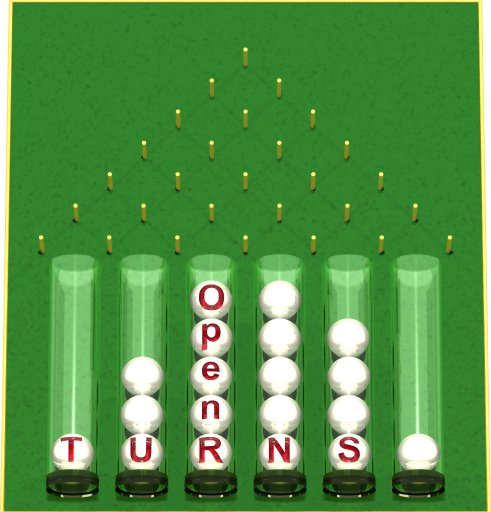
\includegraphics[height=2cm]{logoOT.jpg}
  \end{center}

}

\subject{OpenTURNS Developers Training}

% \part<presentation>{Corps de presentation}


\begin{document}

\frame{\titlepage}

% necessaire pour la table des matieres
\part{Main part}

% table des matieres
\begin{frame}
\Large
  \frametitle{Probabilistic uncertainty propagation}
  \tableofcontents[part=1]
\end{frame}
%%%%%%%%%%%%%%%%%%%%%%%%%%% 
% Uncertainty propagation %
%%%%%%%%%%%%%%%%%%%%%%%%%%% 
\section[What is uncertainty propagation?]{What is uncertainty propagation?}
%%%%%%%%%%%%%%%%%% 
% Main objective %
%%%%%%%%%%%%%%%%%% 
\begin{frame}
  \frametitle{Main objective}
  \begin{block}{Probabilistic uncertainty propagation}
    OpenTURNS = Open Source Treatment of Uncertainty, Risk'N Statistics
    \begin{itemize}
    \item \alert{Uncertainty} = unknown quantities, lack of exact knowledge, non predictible fluctuations
    \item \alert{Risk} = dangerous state, critical conditions and their impact (cost, consequences)
    \item \alert{Statistics} = observation and modelling of random quantities, partial knowledge
    \item \alert{Treatment} = algorithmic tools to analyse, model and quantify the previous points
    \end{itemize}
    The main objective of OpenTURNS is to quantify and analyse a critical \emph{event $E$} built upon a \emph{quantity of interest $Y$} that is linked to \emph{sources of uncertainty $\vect{X}$} through a \emph{numerical model $f$}:
    \begin{equation}
      E=\mathbf{1}_{Y>s}\quad,Y=f(\vect{X})
    \end{equation}
    where $s\in\R$ is a given threshold, $\vect{X}$ is a random vector, $E$ is the critical event. The quantification of this event is typically the evaluation of its \emph{probability of occurence $\P(E)$}.
  \end{block}
\end{frame}
\section[Numerical models: the differential calculus potion]{Numerical models: the differential calculus potion}
%%%%%%%%%%%%%%%%%%% 
% Numerical model %
%%%%%%%%%%%%%%%%%%% 
\begin{frame}
  \frametitle{Numerical models}
  \begin{block}{Function, gradient, hessian}
    \begin{itemize}
    \item \alert{Function:} the notion of \alert{numerical model} is identified with the notion of \alert{numerical function}, it means a function $f$ maps $\R^n$ to $\R^p$. A shortcut is to say that:
      \begin{equation}
        f\in\mathcal{F}(\R^n,\R^p)
      \end{equation}
      The integers $n\in\N$, $p\in\N^{*}$ are the \alert{input} and \alert{output} dimensions. The set $\{\vect{x}\in\R^n|f(\vect{x})\mbox{ is well defined}\}$ is the \alert{domain of definition} of $f$. For all $i\in\{1,\dots,p\}$, the function $f_i\in\mathcal{F}(\R^n,\R)$ defined by $f_i(\vect{x})=\pi_i(f(\vect{x}))$, where $\pi_i$ is the projection on the $i^{th}$ coordinate in $\R^p$, is called the \alert{$i^{th}$ component} of $f$.
    \item \alert{Gradient:} a function $f\in\mathcal{F}(\R^n,\R^p)$ is said to be \alert{differentiable} at $\vect{x}\in\R^n$ if one has:
      \begin{equation}
        \forall\vect{h}\in\R^n, f(\vect{x}+\vect{h})=f(\vect{x})+D(f)(\vect{x})(\vect{h})+o(||\vect{h}||)
      \end{equation}
      where $D(f)(\vect{x})$ is a (continuous) linear application from $\R^n$ to $\R^p$: $D(f)(\vect{x})\in L_c(\R^n,R^p)$. The application $D(f)$ that maps $\vect{x}\in\R^n$ into $L_c(\R^n,R^p)$ is the \alert{differential} of $f$. The linear application $D(f)(\vect{x})$ is always continuous in the setting of $\R^n$ and has an associated matrix $\mat{M}(\vect{x})\in\mathcal{M}_{n,p}(\R)$ whith $M_{ij}=\frac{\partial f_i}{\partial x_j}$: it is the \alert{jacobian matrix} of $f$ at $\vect{x}$. The application that maps $\vect{x}$ into $M^t(\vect{x})\in\mathcal{M}_{p,n}(\R)$ is the \alert{gradient} of $f$ at $\vect{x}$.
    \end{itemize}
  \end{block}
\end{frame}
%%%%%%%%%%%%%%%%%%% 
% Numerical model %
%%%%%%%%%%%%%%%%%%% 
\begin{frame}
  \frametitle{Numerical models}
  \begin{block}{Function, gradient, hessian}
    \begin{itemize}
    \item \alert{Hessian:} a function $f\in\mathcal{F}(\R^n,\R^p)$ is said to be \alert{twice differentiable} at $\vect{x}\in\R^n$ if the application $D(f)$ that maps $\R^n$ into $L_c(\R^n,R^p)$ is differentiable at $\vect{x}$. It means that:
      \begin{equation}
        \forall\vect{h}\in\R^n, D(f)(\vect{x}+\vect{h})=D(f)(\vect{x})+D^2(f)(\vect{x})(\vect{h})+o(||\vect{h}||)
      \end{equation}
      where $D^2(f)(\vect{x})$ is a (continuous) linear application from $\R^n$ to $L_c(\R^n,\R^p)$: $D^2(f)(\vect{x})\in L_c(\R^n,L_c(R^n,R^p))$. The application $D^2(f)$ that maps $\vect{x}\in\R^n$ into $L_c(\R^n,L_c(\R^n,R^p))$ is the \alert{second differential} of $f$. The linear application $D^2(f)(\vect{x})$ is always continuous in the setting of $\R^n$ and has a tensor representation $\mat{T}(\vect{x})\in\mathcal{T}_{n,n,p}(\R)$ whith $M_{ijk}=\frac{\partial^2 f_i}{\partial x_j\partial x_k}$: it is the \alert{second jacobian tensor} of $f$ at $\vect{x}$. The application that maps $\vect{x}$ into $T^t(\vect{x})\in\mathcal{T}_{p,n,n}(\R)$ is the \alert{hessian tensor} of $f$ at $\vect{x}$. This tensor is made of sheets $T_{k,.,.}\in\mathcal{M}_{n,n}(\R)$ that are \alert{symmetric}.
    \end{itemize}
  \end{block}
\end{frame}
\section[A cloud of probabilities in my code, please]{A cloud of probabilities in my code, please}
%%%%%%%%%%%%%%%%%%%%%%%%%%%%%%%%%% 
% Distribution and random vector %
%%%%%%%%%%%%%%%%%%%%%%%%%%%%%%%%%% 
\begin{frame}
  \frametitle{Random vector, distribution}
  \begin{block}{Definition}
    \begin{itemize}
    \item A \alert{random vector $\vect{X}$} is a measurable function from a probability space $(\Omega, \mathcal{B}(\Omega), \P)$ into the probability space $(\R^n,\mathcal{B}(\R^n), \mu_{\vect{X}})$. 
    \item The associated \alert{distribution} is the probability measure $\mu_{\vect{X}}$ defined by:
      \begin{equation}
        \forall B\in\mathcal{B}(\R), \mu_{\vect{X}}(B)=\P(\vect{X}^{-1}(B))
      \end{equation}
    \item The \alert{main advantage} of a random vector is that we are now working on a \alert{numeric space $\R^n$} instead of a general set $\Omega$.
    \item The different values $\forall \omega\in\Omega, \vect{X}(\omega)$ taken by a random vector $\vect{X}$ are called the \alert{realizations} of the random vector.
    \item A distribution is completely defined by its \alert{cumulative distribution function or CDF} $F_{\vect{X}}$ which maps $\R^n$ into $[0,1]$ and is defined by:
      \begin{equation}
        F_{\vect{X}}(\vect{x})=\P(X_1\leq x_1,\dots,X_n\leq x_n)
      \end{equation}
    \end{itemize}
  \end{block}
\end{frame}
%%%%%%%%%%%%%%%%%%%%%%%%%%%%%%%%%% 
% Distribution and random vector %
%%%%%%%%%%%%%%%%%%%%%%%%%%%%%%%%%% 
\begin{frame}
  \frametitle{Random vector, distribution}
  \begin{block}{Discrete random vectors, continuous random vectors}
    There are two distinguished classes of random vectors:
    \begin{itemize}
    \item Those that take their values in $\N^n$ and are called \alert{discrete integral} random vectors. The distribution of this kind of random vectors is equivalently described by the function $p_{\vect{X}}$ that maps $\N^n$ into $[0, 1]$ such that:
      \begin{equation}
        p_{\vect{X}}(\vect{x})=\P(\vect{X}=\vect{x})
      \end{equation}
      The function $p_{\vect{X}}$ is called its \alert{probability distribution function or PDF}.
    \item Those such that there exist a function $p_{\vect{X}}$ that maps $\R^n$ into $R^{+}$ such that:
      \begin{equation}
        F_{\vect{X}}(\vect{x})=\int_{\R^n}p_{\vect{X}}(\vect{x})\,d\vect{x}
      \end{equation}
      These random vectors are called \alert{absolutely continuous} random vectors with respect to the Lebesgue measure $d\vect{x}$. The function $p_{\vect{X}}$ is called its \alert{probability density function or PDF}.
    \end{itemize}
    \begin{description}
    \item[\alert{WARNING 1:}] The PDF acronym is used for two distinct functions, but the context makes it clear which kind of PDF is relevant in practical applications.
    \item[\alert{WARNING 2:}] A random vector can be neither discrete nor continuous!
    \end{description}
  \end{block}
\end{frame}
%%%%%%%%%%%%%%%%%%%%%%%%%%%%%%%%%%
% Distribution and random vector %
%%%%%%%%%%%%%%%%%%%%%%%%%%%%%%%%%%
\begin{frame}
  \frametitle{PDF and CDF, 1D case}
  \begin{tabular}{ccc}
    Continuous & Discrete & General \\
    \fbox{\resizebox{3cm}{!}{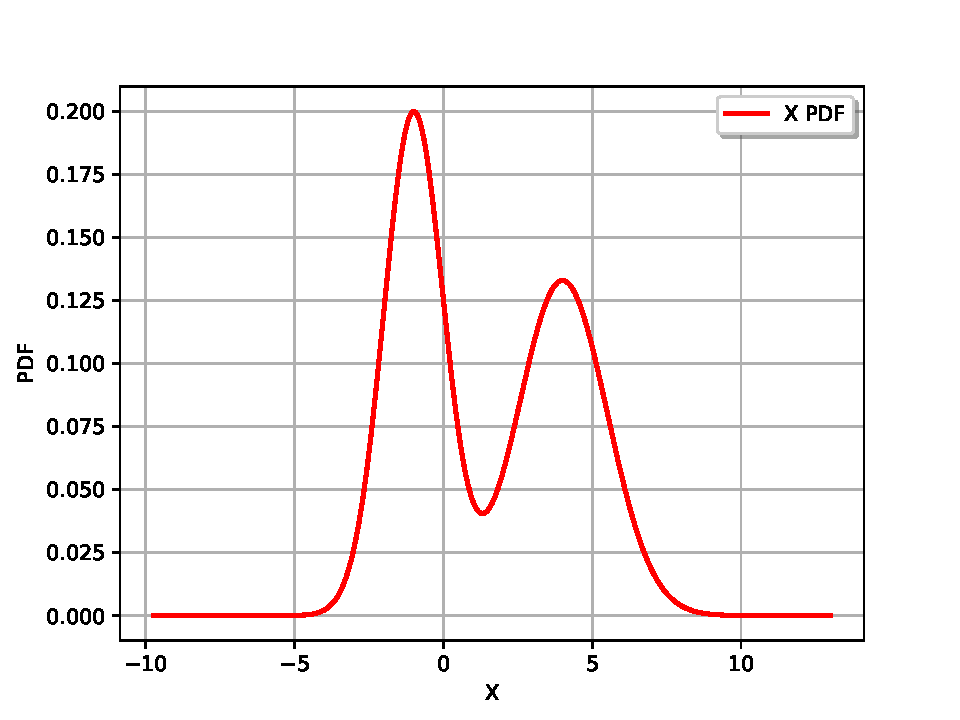
\includegraphics{ContinuousPDF1D.pdf}}} & \fbox{\resizebox{3cm}{!}{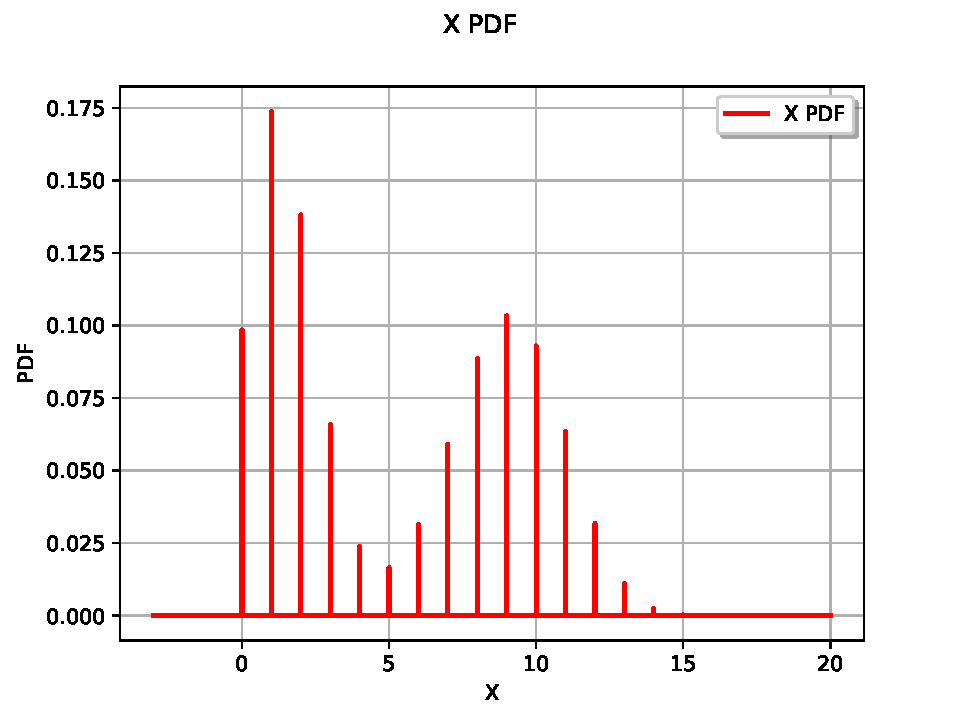
\includegraphics{DiscretePDF1D.pdf}}} & \\[1em]
    \fbox{\resizebox{3cm}{!}{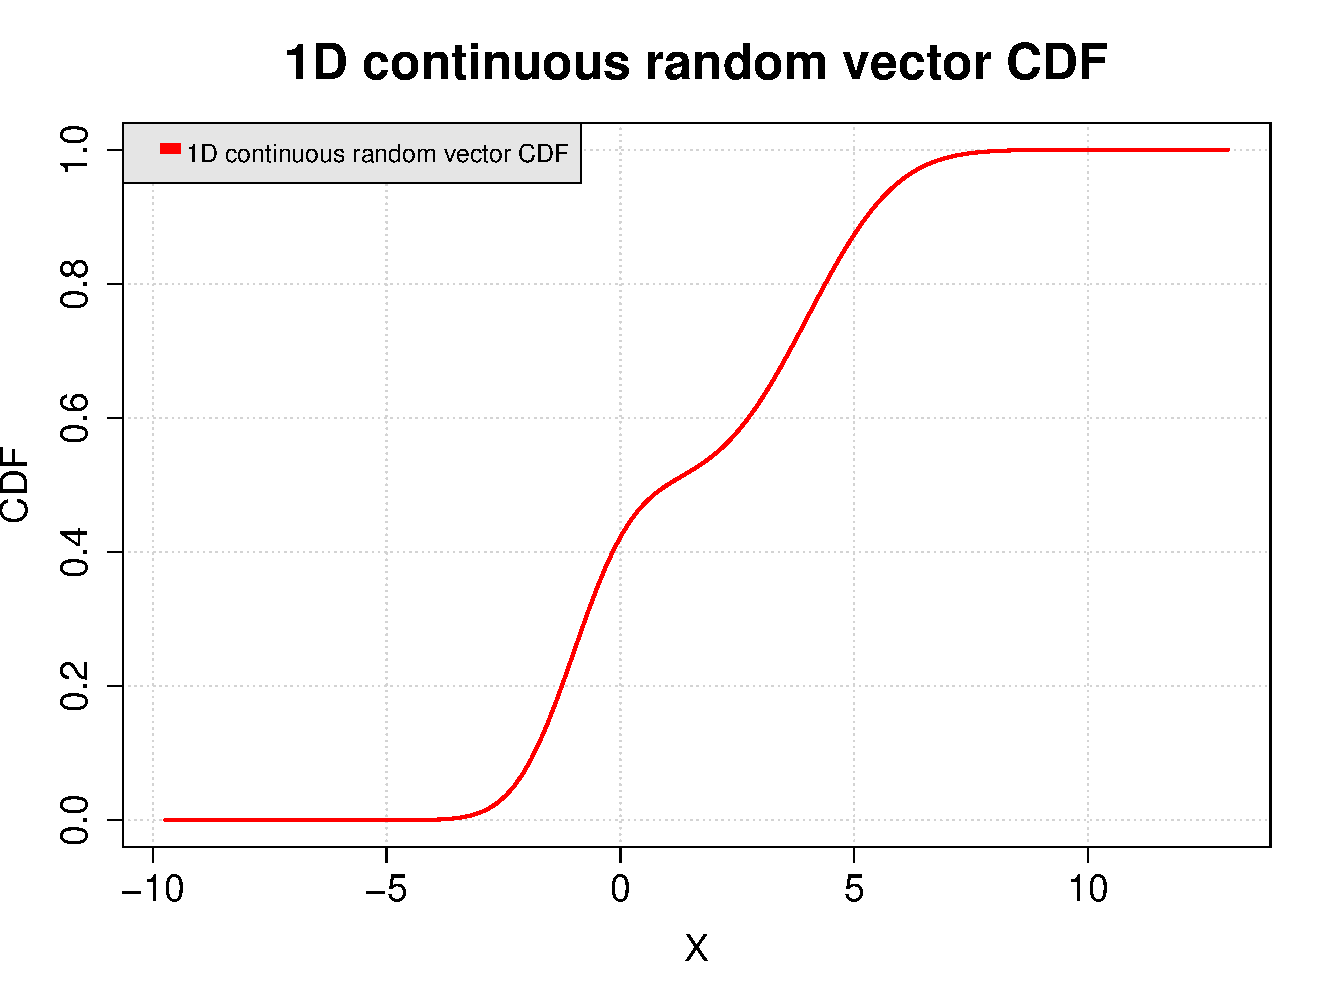
\includegraphics{ContinuousCDF1D.pdf}}} & \fbox{\resizebox{3cm}{!}{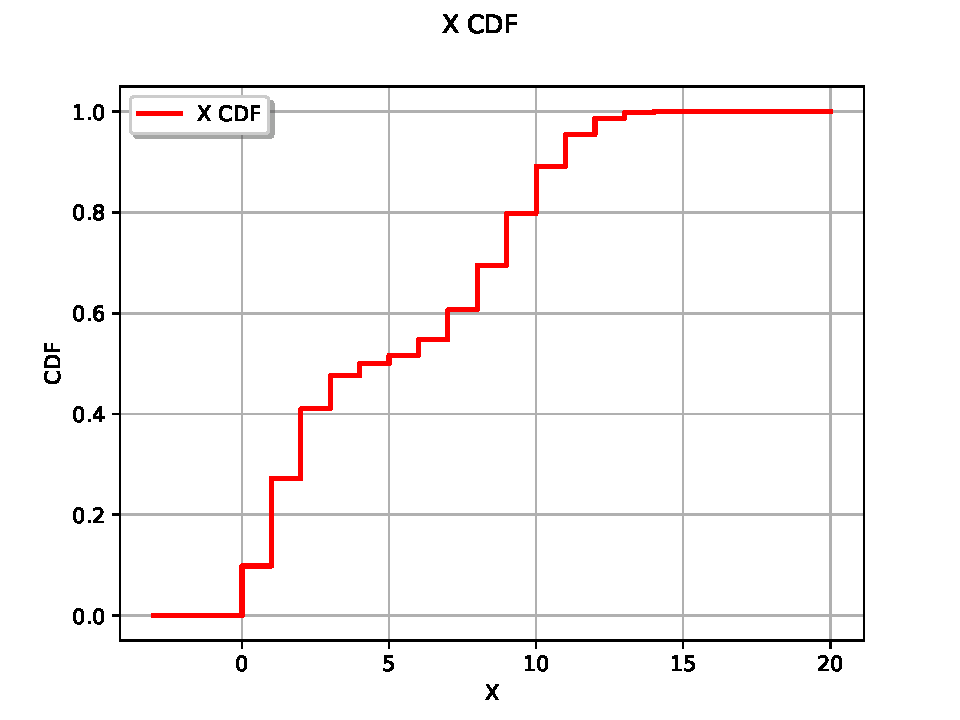
\includegraphics{DiscreteCDF1D.pdf}}} & \fbox{\resizebox{3cm}{!}{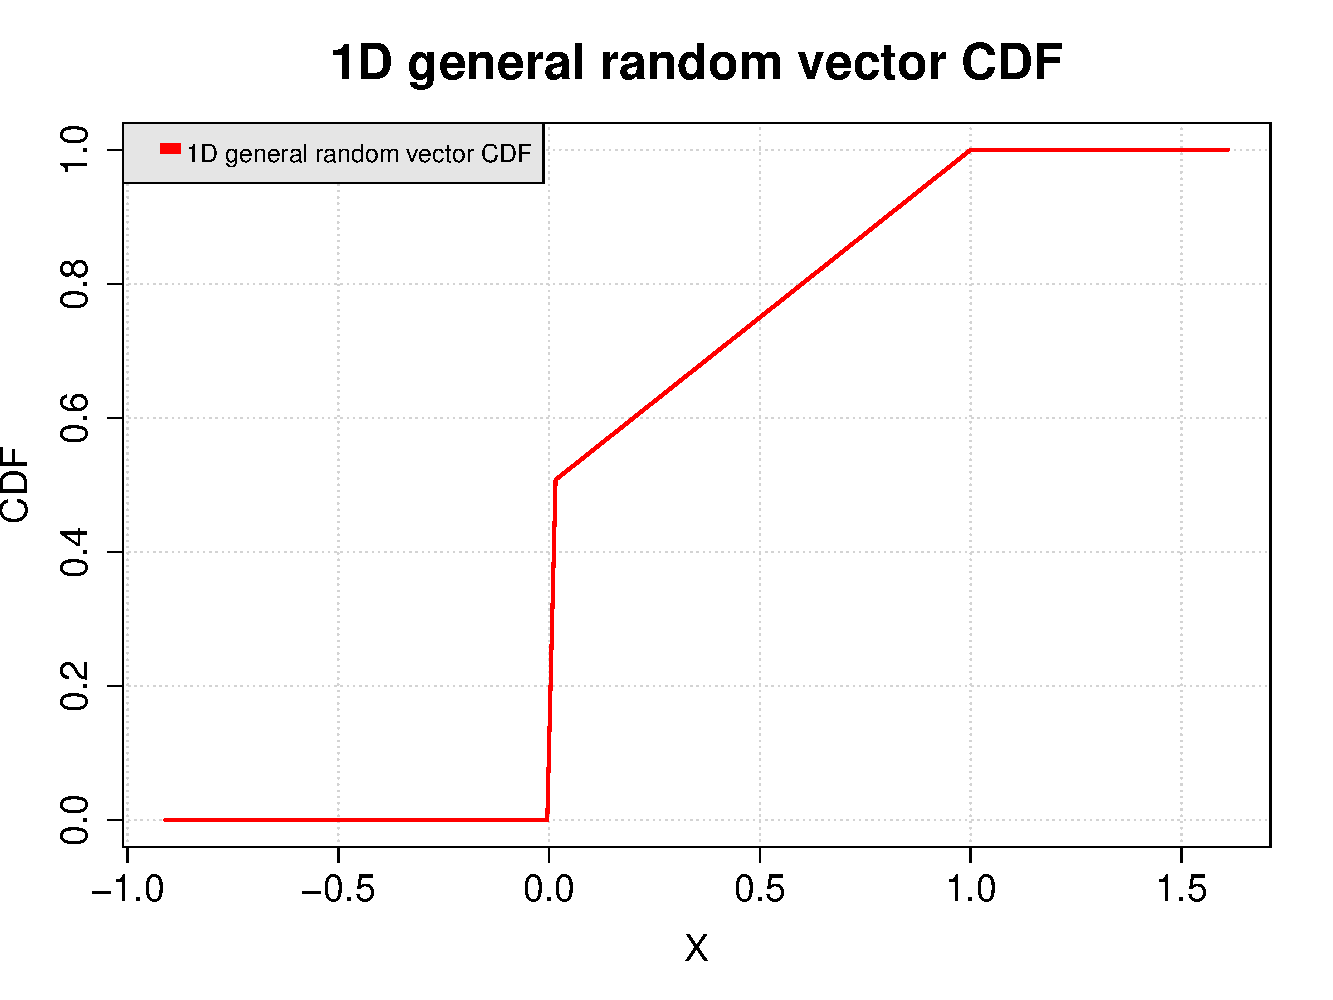
\includegraphics{GeneralCDF1D.pdf}}}
  \end{tabular}
\end{frame}
%%%%%%%%%%%%%%%%%%%%%%%%%%%%%%%%%%
% Distribution and random vector %
%%%%%%%%%%%%%%%%%%%%%%%%%%%%%%%%%%
\begin{frame}
  \frametitle{PDF and CDF, 2D case}
  \begin{tabular}{ccc}
    Continuous & Discrete & General \\
    \fbox{\resizebox{3cm}{!}{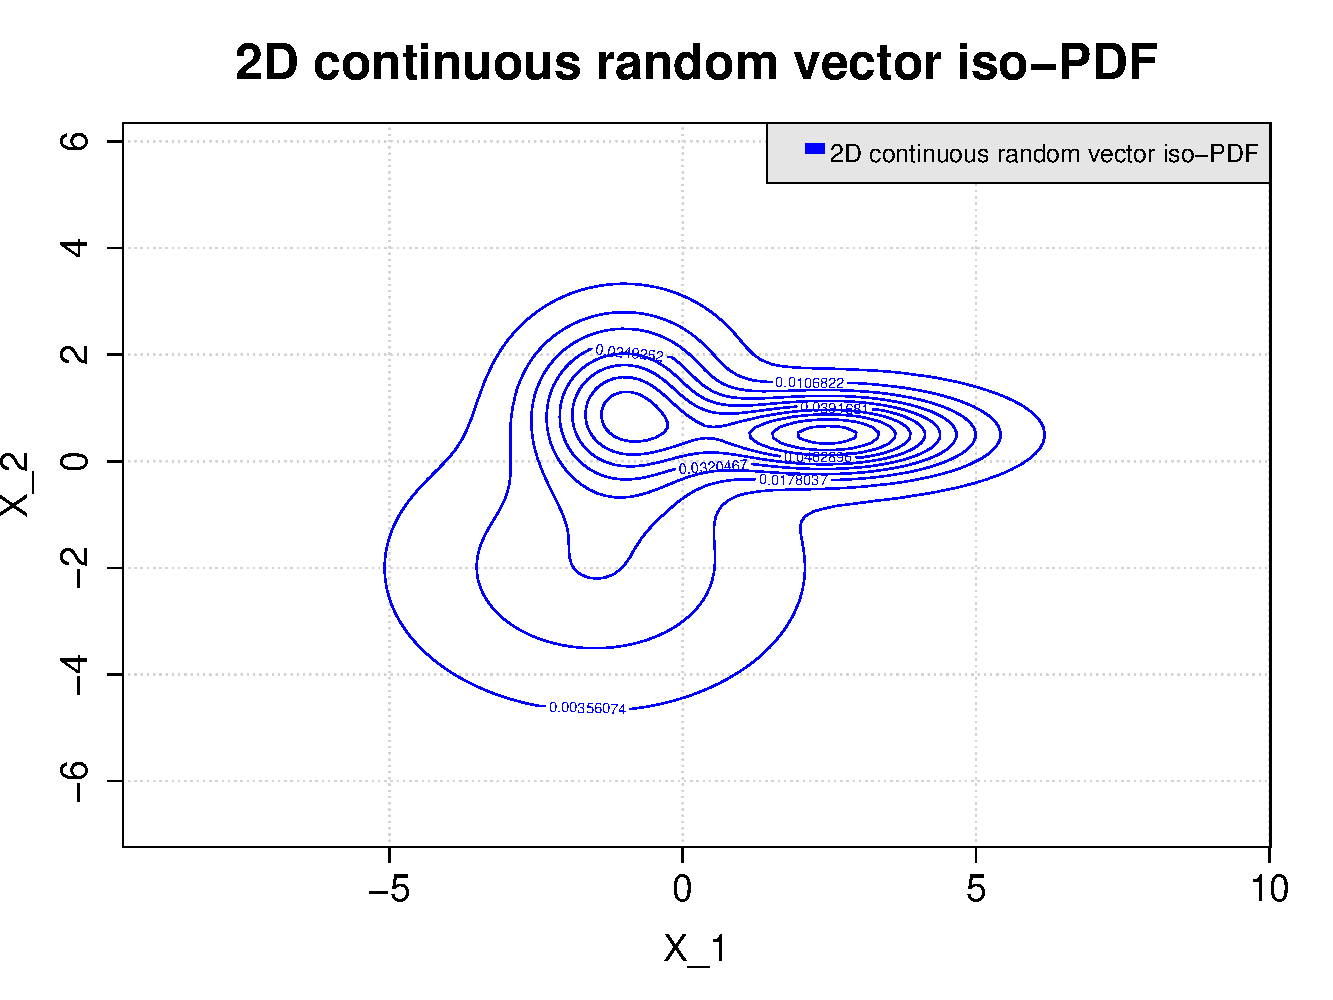
\includegraphics{ContinuousPDF2D.pdf}}} & & \\[1em]
    \fbox{\resizebox{3cm}{!}{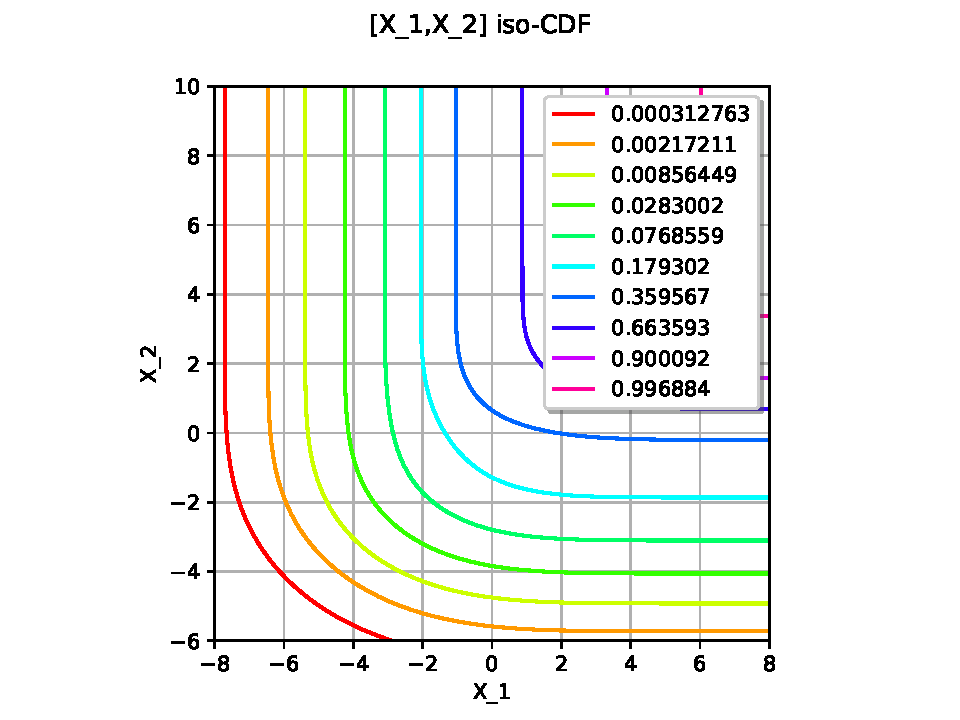
\includegraphics{ContinuousCDF2D.pdf}}} & \fbox{\resizebox{3cm}{!}{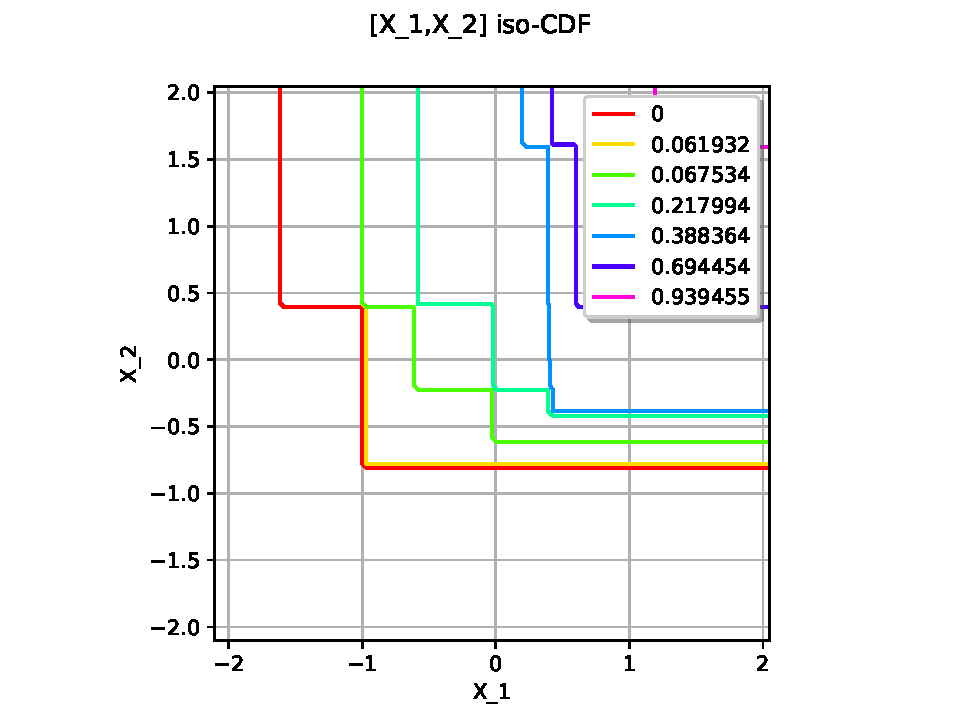
\includegraphics{DiscreteCDF2D.pdf}}} & \fbox{\resizebox{3cm}{!}{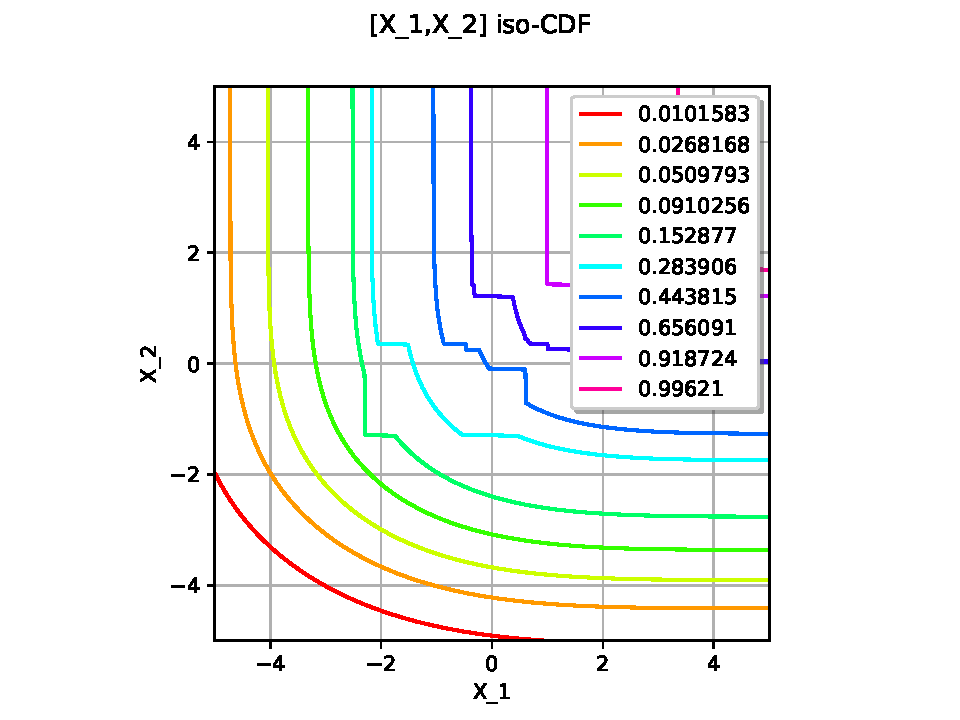
\includegraphics{GeneralCDF2D.pdf}}}
  \end{tabular}
\end{frame}
%%%%%%%%%%%%%%%%%%%%%%%%%%%
% Expectation, Covariance %
%%%%%%%%%%%%%%%%%%%%%%%%%%%
\begin{frame}
  \frametitle{Expectation, mean, covariance}
  \begin{block}{Definition}
    \begin{itemize}
    \item The \alert{expectation $\E[\vect{X}]$} of a real random vector $\vect{X}$ of dimension $n$ is the deterministic vector of $\R^n$ defined by:
      \begin{equation}
        \E[\vect{X}]_i = \int_{\R}x_i\,d\mu_{X_i}(x_i)
      \end{equation}
      where $\mu_{X_i}$ is the distribution of the 1D random vector corresponding to the projection of $\vect{X}$ on its $i^{th}$ coordinate. It is thus a quantity that is defined component by component. For bell shaped distributions, it is an indication of the location of most of the realizations of $\vect{X}$.
    \item The \alert{covariance $\Cov{\vect{X}}$} of a real random vector $\vect{X}$ of dimension $n$ is the deterministic symmetric square matrix of $\mathcal{M}_{n,n}(\R)$ defined by:
      \begin{equation}
        \Cov{\vect{X}}_{ij} = \E[(X_i-\E[X_i])(X_j-\E[X_j])]
      \end{equation}
      where $X_i$ and $X_j$ are the $i^{th}$ and $j^{th}$ components of $\vect{X}$. This matrix is semidefinite positive. For bell shaped distributions, this quantity express the dispersion of the distribution around its mean value.
    \end{itemize}
  \end{block}
\end{frame}
%%%%%%%%%%%%%%%
% Convergence %
%%%%%%%%%%%%%%%
\begin{frame}
  \frametitle{Convergence}
  \begin{block}{Definition}
    \begin{itemize}
    \item A sequence of random vectors $(\vect{X})_{n\in\N}$ defined over the \alert{same} probability space $(\Omega, \mathcal{B}(\Omega), \P)$ is said to \alert{converge almost surely} to the random vector $\vect{X}$ if and only if:
      \begin{equation}
        \P[\{\omega\in\Omega\,|\,\vect{X}_n(\omega)\not\rightarrow\vect{X}(\omega)\mbox{ as }n\rightarrow\infty\}]=0
      \end{equation}
\item A sequence of random vectors $(\vect{X})_{n\in\N}$ defined over the probability spaces $(\Omega_n, \mathcal{B}(\Omega_n), \P_n)$ is said to \alert{converge in law} to the random vector $\vect{X}$ defined over the probability space $(\Omega, \mathcal{B}(\Omega), \P)$ if and only if:
      \begin{equation}
        \forall \phi\in\mathcal{C}^b(\R^n, \R), \lim_{n\rightarrow\infty}\E[\phi(\vect{X}_n)]=\E[\phi(\vect{X})]
      \end{equation}
      where $\mathcal{C}^b(\R^n, \R)$ is the set of bounded continuous functions defined on $\R^n$ and taking value into $\R$.
    \end{itemize}
  \end{block}
\end{frame}
%%%%%%%%%%%%%%
% Simulation %
%%%%%%%%%%%%%%
\begin{frame}
  \frametitle{Simulation}
  \begin{block}{Strong number law and Central Limit Theorem}
    \begin{itemize}
    \item \alert{(Strong law of large numbers)} For all sequence of random vectors $(\vect{X})_{n\in\N}$ defined over the \alert{same} probability space $(\Omega, \mathcal{B}(\Omega), \P)$, \alert{independent} and \alert{sharing the same distribution $\mu_{\vect{X}}$}, for all measurable function $f\in\mathcal{f}(\R^n,\R^p)$ such that $\E[f(\vect{X}_1)]$ exists, \alert{the sequence of random vectors $\left(\frac{1}{n}\sum_{k=1}^nf(\vect{X})\right)_{n\in\N}$ converges almost surely to the constant random vector $\E[f(\vect{X}_1)]$}
    \item \alert{(Central Limit Theorem)} Moreover, \alert{if $\Cov{\vect{X}_1}$ is well-defined and finite}, the sequence of random vectors defined by \alert{$\left(\sqrt{n}\left(\frac{1}{n}\sum_{k=1}^nf(\vect{X})-\E[f(\vect{X}_1)]\right)\right)_{n\in\N}$ converges in law to a multivariate Normal distribution with covariance $\Cov{\vect{X}_1}$}
    \end{itemize}
    The first theorem gives a mean to compute any quantity related to a random vector $\vect{Y}$ defined as the image of a random vector $\vect{X}$ through a numerical model $f$, for exemple its CDF: generate many independent realizations of $\vect{Y}$, take $\phi(\vect{y})=\mathbf{1}_{\{\tilde{\vect{y}}\in\R^p\,|\,\tilde{y}_i\leq y_i}$ and the quantity $\frac{1}{n}\sum_{k=1}^n\phi(\vect{Y})$ will almost surely converge towards $\E[\phi(\vect{Y})]=\P[Y_1\leq y_1,\dots,Y_n\leq y_n]=F_{\vect{Y}}(\vect{y})$. It is the so-called \alert{Monte Carlo method}.\\
    The second theorem gives a mean to quantify the ecision of a Monte Carlo approximation for large but finite values of $n$. As we know the asymptotic behaviour of the fluctuations of $\left(\frac{1}{n}\sum_{k=1}^nf(\vect{X})\right)_{n\in\N}$ we can determine a region $R$ for which the needed quantity has a large probability to be, and we see that this region shrinks with a speed proportional to $\frac{1}{\sqrt{n}}$.
  \end{block}
\end{frame}
%%%%%%%%%%%%%%%
% Monte Carlo %
%%%%%%%%%%%%%%%
\begin{frame}
  \frametitle{Simulation}
  \begin{block}{Monte Carlo algorithm}
    \centering \resizebox{!}{7cm}{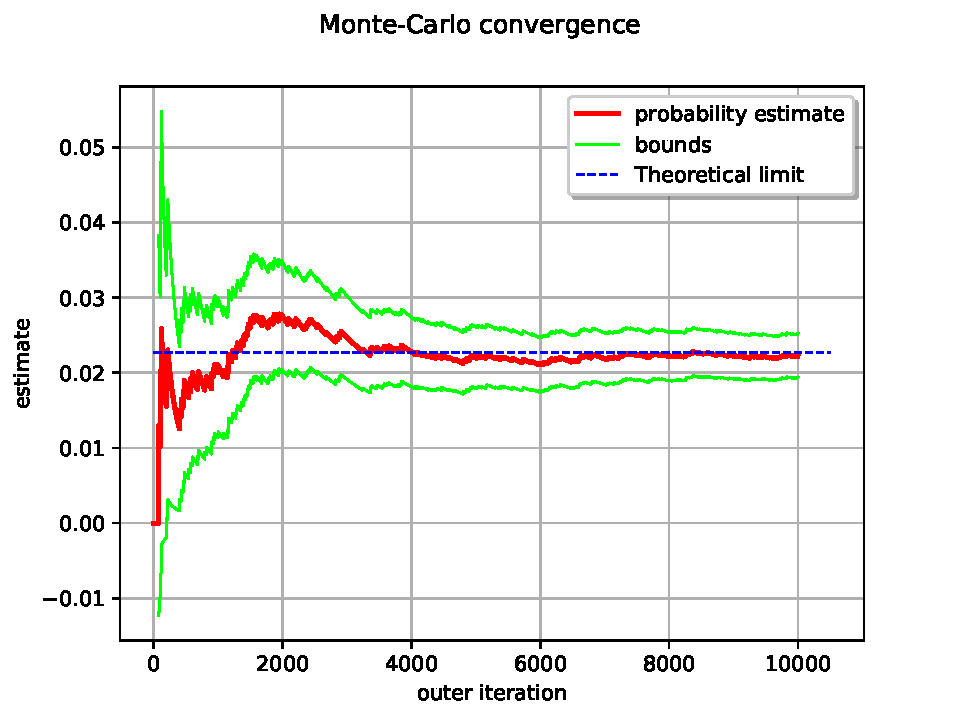
\includegraphics{MonteCarloConvergence.pdf}}
  \end{block}
\end{frame}
%%%%%%%%%%%
% The end %
%%%%%%%%%%%
\begin{frame}
\LARGE
  \frametitle{The end}
  \begin{block}{No more maths!}
    \begin{itemize}
    \item The probabilistic approach to uncertainty propagation involves some high level maths,
    \item The following presentations will show that an OpenTURNS developer must have a basic knowledge of these maths (at least the basic vocabulary) in order to be comfortable with the platform and its objects...
    \item ... but he/she has not to be an expert in order to be efficient!
    \end{itemize}
  \end{block}
\end{frame}
\end{document}

